\documentclass[12pt]{article}

\usepackage{graphicx, color}
\usepackage{setspace}  %espaçamento entre linhas ABNT
\usepackage{indentfirst}
\usepackage{color}
\usepackage{epigraph} %para quem quer colocar epigrafe
\usepackage{todonotes}
%\parindent=15ex
%\oddsidemargin=1cm
%\topmargin=-0.30cm
%\textheight=22.5cm
%\textwidth=15.1cm
%\def \baselinestretch{1.5}
\usepackage{scalefnt} %para mudar o tamanho da fonte
\usepackage{amsmath}
%Pacote Indice remissivo
\usepackage{makeidx}
\usepackage[english]{babel} % pacotes para figura/tabelas...
\usepackage{graphicx, color}
\usepackage{threeparttable}
\usepackage{epigraph} %para quem quer colocar epigrafe
\usepackage[all]{xy}
\usepackage[utf8]{inputenc}
\usepackage{amssymb}
\usepackage{a4wide}
\usepackage{aecompl}
\usepackage{exscale}
% \usepackage{cite}
\usepackage{adjustbox}
\usepackage{booktabs}
%\usepackage[num]{abntcite}
\usepackage[final]{hyperref} % adds hyper links inside the generated pdf file
\usepackage{listings}
\usepackage{titlesec}
\usepackage{biblatex}
\usepackage{rotating}
\usepackage{comment}
\usepackage{color, colortbl}


\hypersetup{
	colorlinks=true,       % false: boxed links; true: colored links
	linkcolor=blue,        % color of internal links
	citecolor=blue,        % color of links to bibliography
	filecolor=magenta,     % color of file links
	urlcolor=blue         
}

%formatacao da section
\titleformat{\section}    
       {\normalfont\fontfamily{phv}\fontsize{16}{17}\bfseries}
       {\thesection.}{0.4em}{}
\titleformat{\subsection}    
       {\normalfont\fontfamily{phv}\fontsize{14}{17}\bfseries}
       {\thesubsection.}{0.1em}{}
       
\titlelabel{\thetitle.\quad}
\titlespacing{\section}{2pt}{20pt}{8pt}
%\titlelabel{\thetitle.\bfseries\quad} %coloca o "." depois.


\pagenumbering{arabic}

\let\oldabstract\abstract
\let\oldendabstract\endabstract
\makeatletter
\renewenvironment{abstract}
{\renewenvironment{quotation}%
               {\list{}{\addtolength{\leftmargin}{0.1cm}
                        \listparindent 0cm%
                        \itemindent    \listparindent%
                        \rightmargin   \leftmargin%
                        \parsep        \z@ \@plus\p@}%
                \item\relax}%
               {\endlist}%
\oldabstract}
{\oldendabstract}
\makeatother

\addbibresource{proposta.bib}

\interfootnotelinepenalty=10000


\graphicspath{{images/}}
\usepackage{subcaption}


\begin{document}
\onehalfspacing
%%%%%%%%%%%%%%%%%%%%%%%%%%%%%%%%% CAPA %%%%%%%%%%%%%%%%%%%%%%%%%%%%%%%%%
%\pagestyle{empty}

\begin{center}
University of São Paulo\\
Institute of Mathematics and Statistics\\
Computer Science Department\\
--\\
\textit{Research Project for the Doctoral Fellowship
\\São Paulo Research Foundation (FAPESP)}\\

\hfill\\

\begin{Large}
    \textbf{Mapping and Mitigating Bottlenecks in the Linux Kernel Development Model}
\end{Large}

\hfill\\

\textbf{Student}: David Tadokoro\\
\textbf{Advisor}: Paulo Meirelles\\
\textbf{Research Internship Abroad advisor}: Gregorio Robles (URJC)\\
\textit{davidbtadokoro@usp.br, paulormm@ime.usp.br, grex@gsyc.urjc.es}
\end{center}


\begin{abstract}
The Linux kernel, a FLOSS project with over 30 years of active development, is central to modern computing. Combined with system tools and utilities from the GNU Project, it forms the GNU/Linux ecosystem, which is fundamental for services in our society, such as the Internet, and ubiquitous in the bleeding edge of fields like Machine Learning. The development of Linux is based on the collaboration of thousands of developers worldwide who interact primarily through email and mailing lists. It is a unique development model involving many processes and practices (workflows) that extend beyond the technical aspects of software development. Despite its success, Linux relies on critical workflows and key personnel, raising concerns about sustainability and workforce renewal. As the codebase and community grow in size and complexity, the entry barrier for newcomers and the workload per maintainer should not increase simultaneously. More interestingly, significant time and resources are spent developing tools that address limitations in the Linux kernel development model that the practitioners feel in their day-to-day work, yet these challenges are underexplored in academia. This research project aims to: 1) propose taxonomies that accurately detail the workflows that define the Linux kernel development model and identify inherent bottlenecks; 2) mitigate bottlenecks by developing FLOSS tools that support the Linux ecosystem.\\

\textbf{Keywords}: Linux, FLOSS, Linux kernel development model, FLOSS development model, bottleneck mitigation, software engineering.

\end{abstract}

\section{Introduction}
\label{chp:introduction} 

Computers, ranging from personal devices to embedded systems in automobiles, are essential in modern life and typically consist of hardware (physical components) and software (programs controlling the hardware). A key software component is the Operating System (OS), which acts as a bridge between hardware and software, with its kernel being the core program managing hardware details and enabling other programs to function~\cite{silberschatz2008-operatingsystemconcepts}. The Linux kernel, a Free/Libre/Open Source Software (FLOSS), exemplifies this by being highly customizable and widely used across various sectors, including Internet infrastructure and machine learning, making it a critical solution for real-world problems. Its adaptability and lack of licensing costs have made it central to the technology industry, supported by diverse stakeholders.

\subsection{The Linux kernel FLOSS ecosystem}

The Linux kernel project is structured into interconnected subsystems, analogous to neighborhoods in a city~\cite{wen2021-masterthesis}, each managed by maintainers who oversee contributions from developers. The \texttt{MAINTAINERS} file lists maintainers and their respective codebase portions. However, entries in the \texttt{MAINTAINERS} file often overlap and share code, forming clusters rather than isolated entities that more closely represent subsystems~\cite{corbet2021-subsystems}. The Linux community operates in a decentralized, global, and asynchronous manner, reflecting its distributed nature. Figure~\ref{fig:linux-subsystems} illustrates this complexity, showing an undirected graph of \texttt{MAINTAINERS} entries and their codebase overlaps, highlighting the interconnection of subsystems.


\begin{figure}[ht]
    \centering
    \begin{subfigure}[b]{0.3\textwidth}
        \centering
        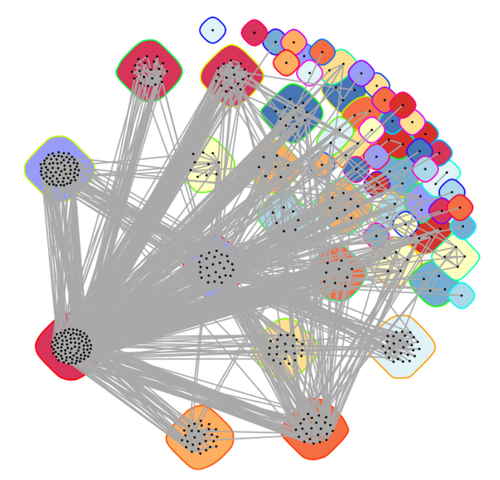
\includegraphics[width=1\textwidth]{images/linux-subsystems.png}
        \caption{Clusters of the \texttt{MAINTAINERS} file.\label{fig:linux-subsystems}}
    \end{subfigure}
    \begin{subfigure}[b]{0.3\textwidth}
        \centering
        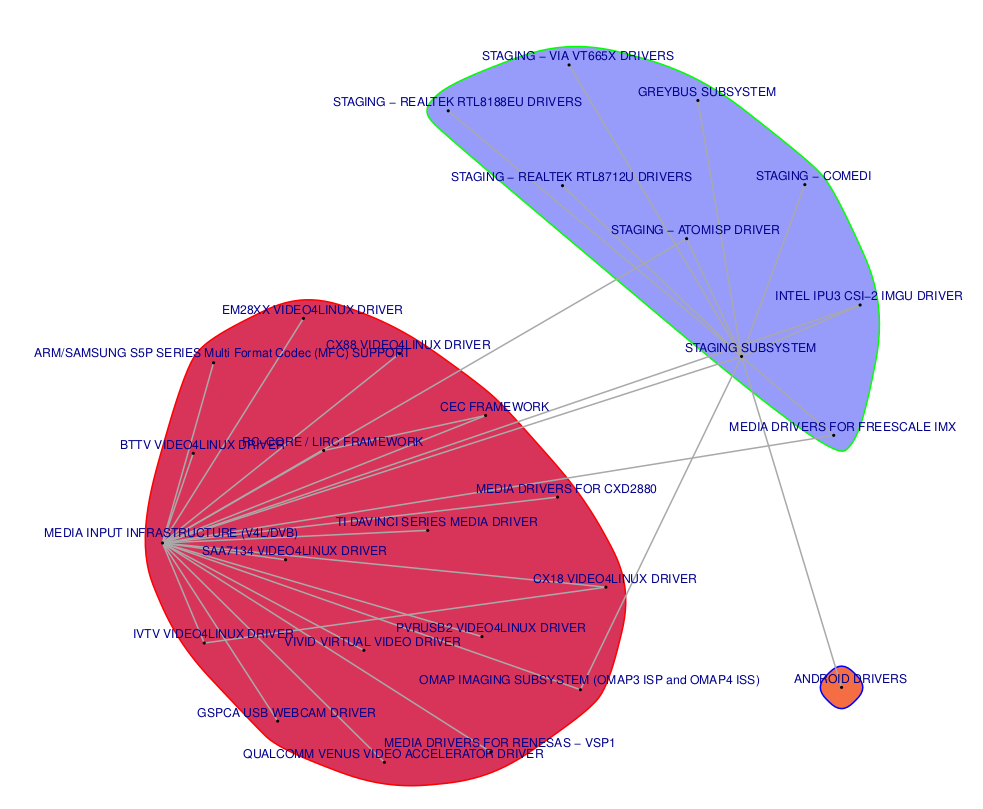
\includegraphics[width=1\textwidth]{images/media-subsystem.png}
        \caption{\textit{media} subsystem\label{fig:media-cluster}}
    \end{subfigure}
    \begin{subfigure}[b]{0.3\textwidth}
        \centering
        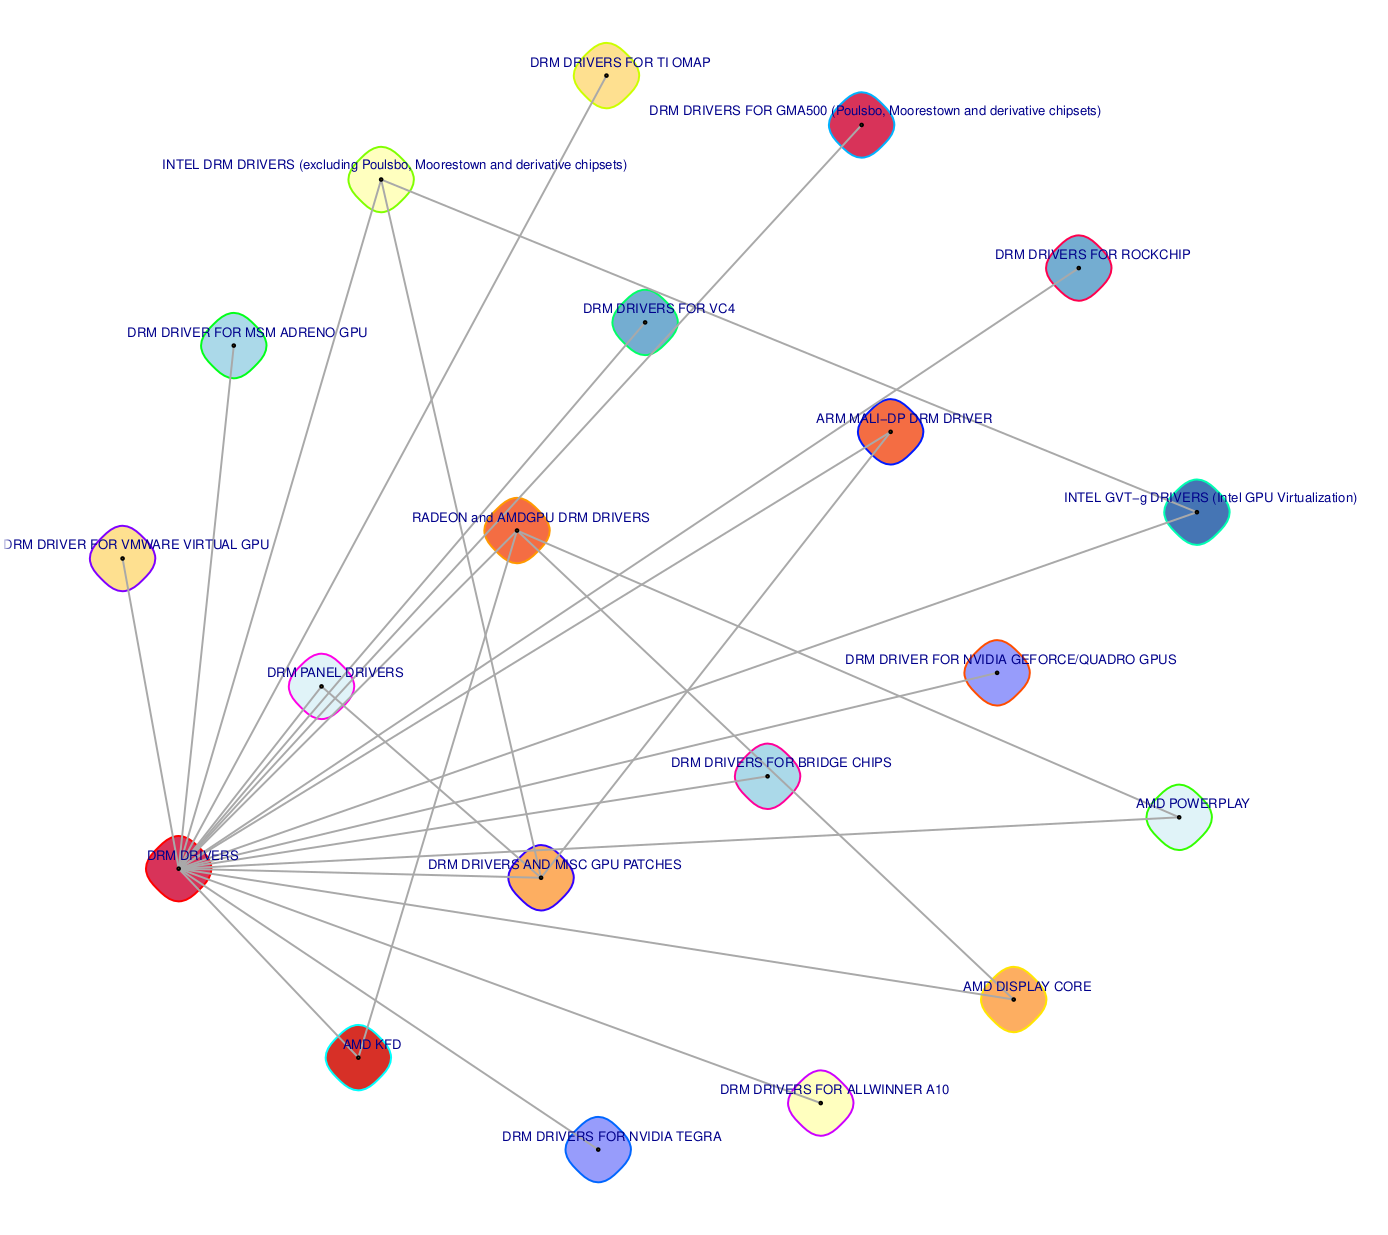
\includegraphics[width=1\textwidth]{images/drm-subsystem.png}
        \caption{\textit{DRM} subsystem\label{fig:drm-cluster}}
    \end{subfigure}
    \caption{Subsystems of the Linux kernel. \textit{Source} ~\cite{corbet2021-subsystems}.\label{fig:linux-clusters}}
\end{figure}

Despite their coupling, each subsystem has unique governance, maintainership models, and domain-specific characteristics. Figures~\ref{fig:media-cluster} and \ref{fig:drm-cluster} provide a closer look at the \textit{media} and \textit{DRM} subsystems, respectively, showcasing their distinct organizational structures. These examples underscore the diversity within the Linux kernel subsystems, even as they remain deeply interconnected~\cite{wen2021-masterthesis}.

\subsubsection{How the Linux kernel subsystems connect}

As mentioned, the Linux kernel project operates like a city divided into neighborhoods (subsystems), each governed by maintainers and supported by their ecosystems. These subsystems manage specific codebase portions within a hierarchical \textit{web of trust}, where upper levels delegate tasks to lower levels. Linus Torvalds, the creator of Linux, sits at the top as a \textit{benevolent dictator} \cite{corbet2014-4.4}, resolving disputes and overseeing the project. Despite this hierarchy, the structure is flatter than it seems, with most maintainers submitting pull requests\footnote{A request to merge changes made in one fork of a project into the original repository. Not to be confused with \textit{GitHub Pull-Requests}.} directly to Linus, bypassing mid-level maintainers \cite{corbet2017-patchflow}. While scalable, this model has led to inefficiencies, such as 44\% of contributions being ignored over the past decade \cite{rigby2014-peer-review}, causing frustration and wasted effort within the community.

\begin{figure}[ht]
    \centering
    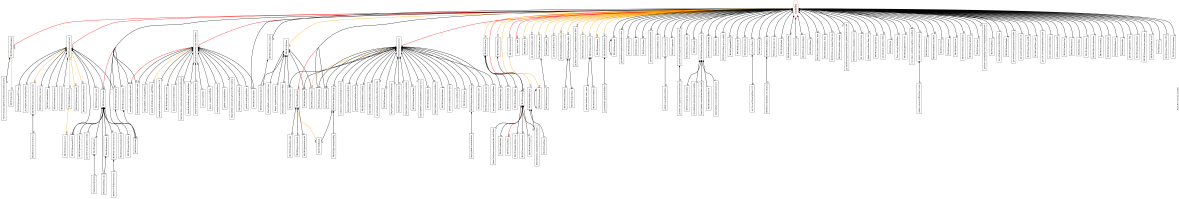
\includegraphics[width=1\textwidth]{images/treeplot-4.4-full-sm-fixed.png}
    \caption{Flow of changes from the Linux 4.4 development cycle as a tree plot showing the flat hierarchy of the development model (this figure is not supposed to be readable). \textit{Source}:~\cite{corbet2014-4.4}.\label{fig:4.4-hierarchy}}
\end{figure}

Subsystems function as independent projects with their own forks, synchronizing with the \textit{mainline} (Linus' tree) via pull requests. This decentralized model offers flexibility but creates dependencies on key maintainers, particularly Linus. Figure~\ref{fig:4.4-hierarchy} depicts the flat hierarchy of the Linux 4.4 development cycle, emphasizing Linus' central role and the ecosystem interconnection. Although this structure has driven Linux success, it exposes vulnerabilities, such as maintainer overload and reliance on critical individuals, which could threaten the project long-term sustainability.

\subsubsection{Patches and the Linux kernel development process}

At the heart of the Linux kernel development process is the \textit{patch}, a text document that describes changes between two versions of a source tree and represents a contribution to the project \cite{wen2021-masterthesis}. Similar to a git commit, a patch includes a code differential and a descriptive message but is formatted for email submission via mailing lists. Development, bug reporting, and discussions occur on these lists, with contributors submitting patches for review. Maintainers and the community provide feedback, leading to iterative revisions in a process known as the \textit{patch-reviewing process}. This back-and-forth ensures high-quality contributions \cite{palix2011-faults-linux}, and once a patchset (set of patches that comprise a contribution) is deemed ready, it begins its journey through the upstream (upper levels of Linux hierarchy) repositories.

\begin{figure}[ht]
    \centering
    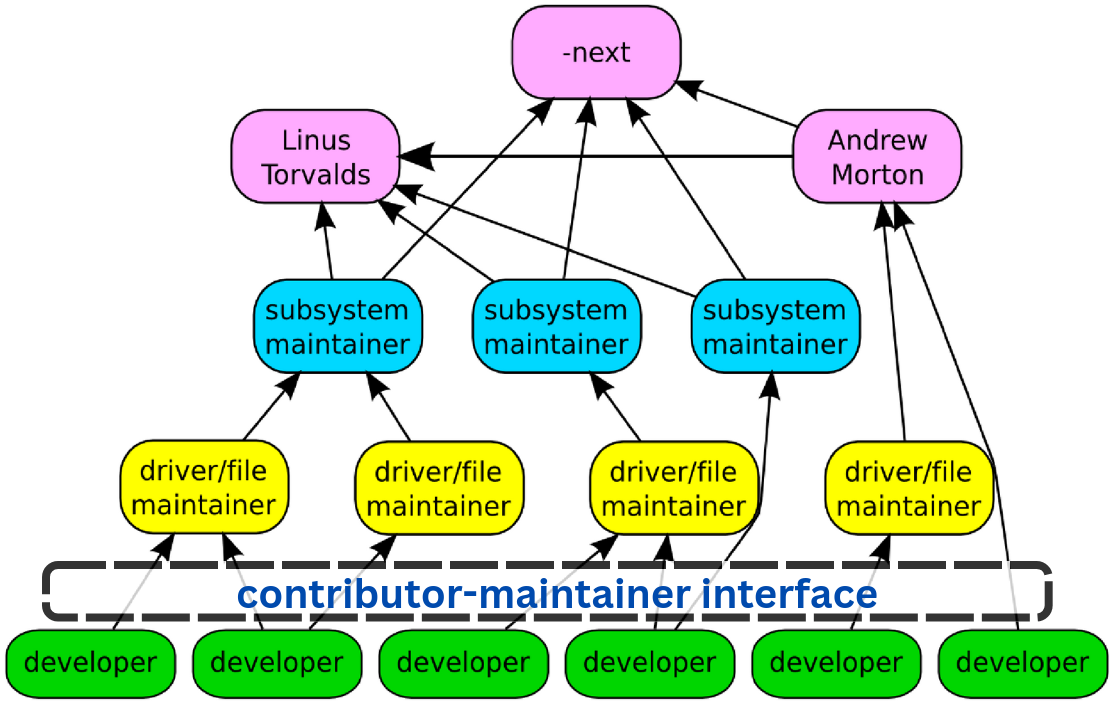
\includegraphics[width=0.4\textwidth]{images/patch-lifecycle.png}
    \caption{Patches flow into the \textit{mainline}. \textit{Source}:~\cite{gregkh2016-patches-carved}.\label{fig:patch-lifecycle}}
\end{figure}

Patches are first merged into the subsystem official repository, where maintainers have jurisdiction, and then progress up the hierarchy until they reach Linus Torvalds in the \textit{mainline} repository. Figure \ref{fig:patch-lifecycle} illustrates this flow, showing how patches move from contributors to the mainline. Along the way, \textit{Continuous Integration} (CI) practices, such as stabilization in \texttt{-next} branches, ensure changes do not destabilize the project. For example, the \textit{AMD DRM} subsystem uses the \texttt{amd-staging-drm-next} branch for this purpose.

Despite its effectiveness, the patch and email-based development process is considered outdated. \textit{Izquierdo-Cortazar et al. (2017)} \cite{izquierdo2017-review} argue for modernizing the review process, as mailing lists require proactive subscription and often face delivery issues. Tools like the Lore kernel archives and \textit{GitGitGadget} aim to address these challenges by providing real-time web access to mailing lists and enabling contributions via \textit{GitHub Pull-Requests}, respectively. These efforts highlight the need to adapt the Linux development model to contemporary standards while maintaining its collaborative and decentralized nature.

\subsubsection{The Linux kernel development model}

The Linux kernel development model encompasses a variety of \textit{workflows} that extend beyond technical functionalities, including practices like submitting patches to mailing lists, adhering to subsystem-specific rules, and following strict development cycles. These workflows are essential for maintaining the project structure and quality but also reveal bottlenecks that hinder efficiency. As noted by \textit{Corbet and Kroah-Hartman (2017)} \cite{corbet-gregkh2017-linuxreport}, tools are critical for managing the complexity of a project as large as Linux. For instance, git, created by Linus Torvalds in 2005, replaced the previous version control system and has since become indispensable for developers worldwide.

To address these bottlenecks, the Linux community develops tools ranging from official scripts like \texttt{get\_maintainers.pl} (finds patch recipients) to standalone projects like \texttt{b4} (fetches patches from archived mailing lists). Many developers also create personal scripts to solve specific issues, leading to duplicated efforts and a lack of systematic cataloging of solutions. Researchers involved in this project are actively developing FLOSS tools, such as the \textit{kworkflow}\footnote{\href{https://kworkflow.org}{https://kworkflow.org}} project and its subproject \textit{patch-hub}. These tools aim to unify solutions under a single interface, reducing inefficiencies and improving the overall development experience.

\subsection{Problem outline}

On one hand, the Linux kernel project steadily grows in size, complexity, and number of developers involved. On the other hand, we can name a few of the concerns about its development model detected by academia and practitioners:
(i) Scalability of the community and the workflows; 
(ii) Renewal of the workforce;
(iii) Key personnel that occupy critical roles and are often irreplaceable;
(iv) Waste of community effort and resources;
(v) Inefficient and outdated technologies that are at the core of the model;
(vi) \textit{Ad-hoc} solutions to workflow bottlenecks and duplication of work.


More severely, academic studies on the Linux project mostly detach from observing the practice and lack a proper investigation of these matters, carrying homogeneous and biased views~\cite{wen2021-masterthesis}. As a result, there are misleading conclusions from the academic that surface when contrasted with the perspective of the Linux community (\textit{Grey Literature}) and with the close observation of the practice (\textit{ethnographic case-studies}) \cite{wen2021-masterthesis}. We also point out that the ubiquity of \textit{ad-hoc} solutions to bottlenecks general to most Linux developers has an impact on the scalability of workflows and the workforce and compromises the project sustainability in the long term; therefore, in-depth academic research into the Linux ecosystem that unifies state-of-the-art and state-of-the-practice can lead to informed decisions on the development of critical tools that support the Linux umbrella project.

\section{Objectives}
\label{chp:objectives}

Given the gap in the academic understanding of the Linux kernel development model when contrasted with the practice, there are undoubtedly several topics that are either not covered at all or investigated in a shallow manner by academic literature. For instance, in the Linux community, there is a quasi-mature discussion about the social challenges, and actions are taken in that regard, like a self-imposed break by Linus Torvalds \cite{linus2018-stepdown} after strong disagreements with the community. There is even a \textit{Code of Conduct} (CoC) \footnote{\href{https://www.kernel.org/doc/html/latest/process/code-of-conduct.html}{Permalink to latest Code of Conduct file}.} that has a committee to handle reported misconduct. Nevertheless, no academic studies covered these topics at all \cite{wen2021-masterthesis}.

Even though social challenges are significant - after all, software engineering considers the process of developing software as a socio-technical phenomenon - this proposed project focuses on understanding the overarching workflows (i.e., the processes and practices) that define the Linux kernel development model.
%
In this sense, we present the two primary objectives of this work:

\begin{itemize}
	\item \textbf{Objective 1}: Validate a theoretical framework that accurately describes the overarching workflows of the Linux kernel development model and allows us to identify bottlenecks;
	\item \textbf{Objective 2}: Develop FLOSS tools that efficiently mitigate bottlenecks in the Linux kernel development model using informed decisions based on a validated theoretical framework.
\end{itemize}

We acknowledge that successfully reaching these objectives does not directly solve all the previously outlined problems. Nonetheless, it does serve as a starting point for ans-wering them.
%
To fulfill these objectives, we will adopt a multi-method approach focusing on \textit{ethographic case-studies} to be close to the practice while also considering the academic literature, grey literature, and community perspectives to triangulate findings and fortify their accuracy.
%
To guide the research, we present three questions:

\begin{enumerate}
    \item \textbf{RQ.1}: What overall workflows compose the Linux kernel development model?
    \item \textbf{RQ.2}: Which processes and/or practices generate bottlenecks in the Linux kernel development model that compromise its efficiency and scalability?
    \item \textbf{RQ.3}: Which bottlenecks can be mitigated by streamlining processes through automation?
\end{enumerate}

\subsection{Expected and preliminary results}

In \textbf{Objective 1}, we aim to validate a taxonomy within the framework of \textit{Grounded Theory} (GT), which involves constructing a structured classification system based on empirical data~\cite{glaser2017-grounded} and its use has become commonplace in the software engineering field~\cite{leite2022-master}. The produced taxonomy will categorize the macro workflows in Linux kernel development, potentially including nested subcategories for finer-grained analysis. Over time, this taxonomy is expected to evolve into an \textit{emergent theory}, a coherent explanatory framework that extends beyond mere classification. This emergent theory will provide a mature and solid foundation for understanding and deriving conclusions about the Linux kernel development model, offering insights into its complexities and workflows.

\begin{figure}[ht]
    \centering
    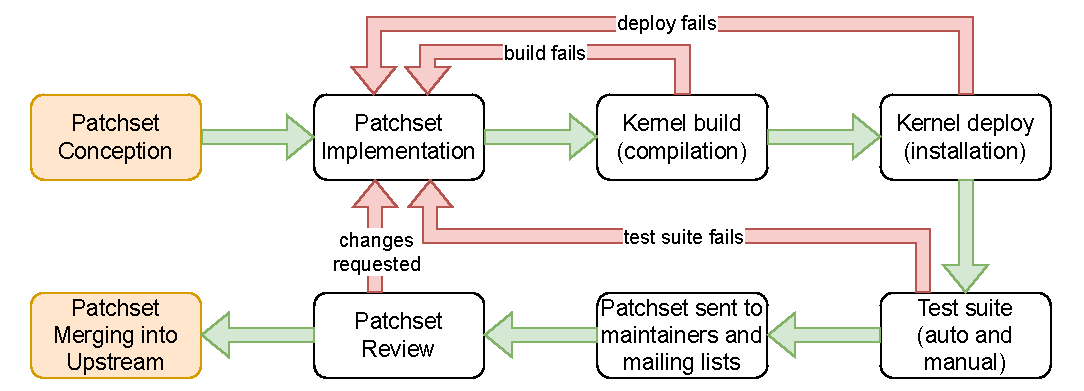
\includegraphics[width=0.8\textwidth]{images/patch-development-workflow.pdf}
    \caption{Concept map of the patchset-development workflow.\label{fig:patch-development-workflow}}
\end{figure}


Figures \ref{fig:patch-development-workflow} and \ref{fig:patchset-reviewing-workflow} illustrate two key workflows in Linux development. Figure \ref{fig:patch-development-workflow} depicts the patchset-development workflow, which spans from the conception of a contribution to its submission, review, and start of merging into the upstream. It includes technical processes like kernel compilation and deployment, as well as practices such as sending patches to the correct maintainers and participating in the review process. Figure \ref{fig:patchset-reviewing-workflow} focuses on the patchset-reviewing workflow, which is more relevant to maintainers. It outlines steps from fetching and selecting patchsets to providing feedback or initiating the merging process. Both workflows highlight the interactive and collaborative nature of Linux development, with variations depending on the subsystem and development context. These concept maps were derived from \textit{Participant Observation}, where the doctoral student: (i) contributed to subsystems like \textit{AMD GPU}, \textit{Industrial I/O}, and \textit{staging}; (ii) developed and maintained tools that support the community; (iii) mentored newcomers into Linux development.

\begin{figure}[ht]
    \centering
    \includegraphics[width=0.6\textwidth]{images/patchset-reviewing-workflow.png}
    \caption{concept map of the patchset-reviewing workflow.\label{fig:patchset-reviewing-workflow}}
\end{figure}


The doctoral student's ongoing development of FLOSS tools to support the Linux ecosystem aligns with \textbf{Objective 2}. By leveraging insights from the taxonomy iterations, informed decisions can be made to address bottlenecks and improve workflows. These tools, such as those aiding patch submission and review, aim to streamline processes and enhance efficiency within the Linux development model. This iterative approach ensures that the tools are grounded in the realities of the Linux ecosystem, addressing actual needs identified through systematic analysis.



\section{Justification}
\label{chp:justification}

Our research group has extensive experience with the Linux ecosystem, including current and past members who have actively contributed to subsystems such as \textit{AMD GPU}, \textit{Industrial I/O (IIO)}, and \textit{Virtual Kernel Mode Setting} (VKMS). Many of these members work professionally as contributors and maintainers, dedicating themselves entirely to Linux development. For instance, our students accounted for 20\% of all accepted contributions to the IIO subsystem during a 90-day period in 2019. Drawing from this experience, our group developed a FLOSS project called \textit{kworkflow} (\textit{kw}), a \textit{Developer Automation Workflow System} (DAWS) designed to streamline and automate workflows for Linux developers.

\textit{kworkflow}\footnote{\href{https://kworkflow.org}{kworkflow site} and \href{https://github.com/kworkflow/kworkflow/}{kworkflow repository}.} provides a unified interface offering solutions to common kernel development challenges, such as abstracting hardware and distribution-specific complexities for tasks like configuring, compiling, and installing custom kernels. It also includes tools for submitting contributions and managing reviews, which have gained traction among industry developers. In 2023, the doctoral student became a maintainer of \textit{kworkflow} and the primary maintainer of its subproject, \textit{patch-hub}\footnote{\href{https://github.com/kworkflow/patch-hub/}{patch-hub repository}.}. This \textit{Terminal User Interface} (TUI), designed for maintainers, simplifies interaction with contributions sent to mailing lists and review management, addressing one of the most critical bottlenecks in the development model.

Our firsthand experience and continuous interaction with researchers and practitioners have generated valuable insights. By systematically mapping Linux kernel development workflows and identifying bottlenecks, we aim to bridge the gap between theory and practice, opening avenues for future research and potentially applying these findings to other software engineering contexts. Pragmatically addressing these bottlenecks with high-quality tools will benefit the Linux ecosystem - contributors, maintainers, testers, and other stakeholders - by streamlining complex processes, enhancing productivity, reducing workload, increasing contribution throughput, and scaling the workforce. Ensuring these tools are FLOSS is crucial, as it allows the Linux community to provide feedback and contribute organically, aligning with \textbf{Objective 2}.

Additionally, addressing these challenges could free up resources to tackle underprioritized issues, such as the project environmental sustainability. Given Linux pervasive role in technology - from embedded systems and Internet infrastructure to supercomputers and AI machine learning model training - making it more environmentally friendly could have a significant global impact. Furthermore, improving Linux quality as a software solution could create a positive ripple effect across modern computing, reinforcing its importance as a cornerstone of FLOSS development.

\subsection{Evidence about the gap in academic understandings of the Linux kernel development model}

A symptom of the misleading conclusions from the scientific community about the Linux kernel development model is the divergent definitions given by different authors.

For \textit{Rigby et al. (2014)}~\cite{rigby2014-peer-review}, the model is a dictatorship that relegates newcomers and has a rigid and subservient culture; For \textit{Fogel (2017)}~\cite{fogel2017-producing-oss}, the ``forkability'' of the project results in a ``benevolent dictator'' model where Linus does not have full authority on the project; \textit{Lindberg et al. (2014)}~\cite{lindberg2014-theorizing}, believes that a core group of developers takes most of the reviews and is also exclusively responsible for approving code changes, following a \textit{Cathedral model}~\cite{raymond1999-cathedral}; finally, \textit{Shaikh and Henfridsson (2017)}~\cite{shaikh2017-governing-oss} argue that four governance types coexist in the Linux kernel development: autocracy, oligarchy, federation, meritocracy.

The lack of a consensus on a primordial aspect, such as categorizing the Linux kernel development model, indicates how academic investigations are at an early stage. At last, \textit{Wen (2021)}~\cite{wen2021-masterthesis}, using the qualitative research method of \textit{Directed Content Analysis}, produced mind maps that describe the Linux kernel development model. They showed, at large, gaps and misconceptions from the scientific community when crossed with community perspectives. 

\subsection{Empirical evidence about the unsustainability of the Linux kernel development model}

We have produced empirical quantitative evidence indicating that the Linux kernel development model may be unsustainable due to its current structure\footnote{These experiments are reproducible with \textit{Docker} following the instructions in \href{https://github.com/davidbtadokoro/phd-experiments/tree/master/linux-stats}{this repository}.}. Figures \ref{fig:loc-linux}, \ref{fig:maintainers-linux}, and \ref{fig:commits-linux} are plots that show statistics about the development of Linux over the last 10 years. Due to the periodicity of releases that follow subsequent six to eight-week cycles, we can use the Linux versions as consistent timestamps to analyze the evolution of the project. In this sense, the aforementioned figures have the Linux versions in the abscissa from 3.19 (launched on 8 February 2015) until 6.13 (launched on 20 January 2025).

\begin{figure}[h!]
    \centering
    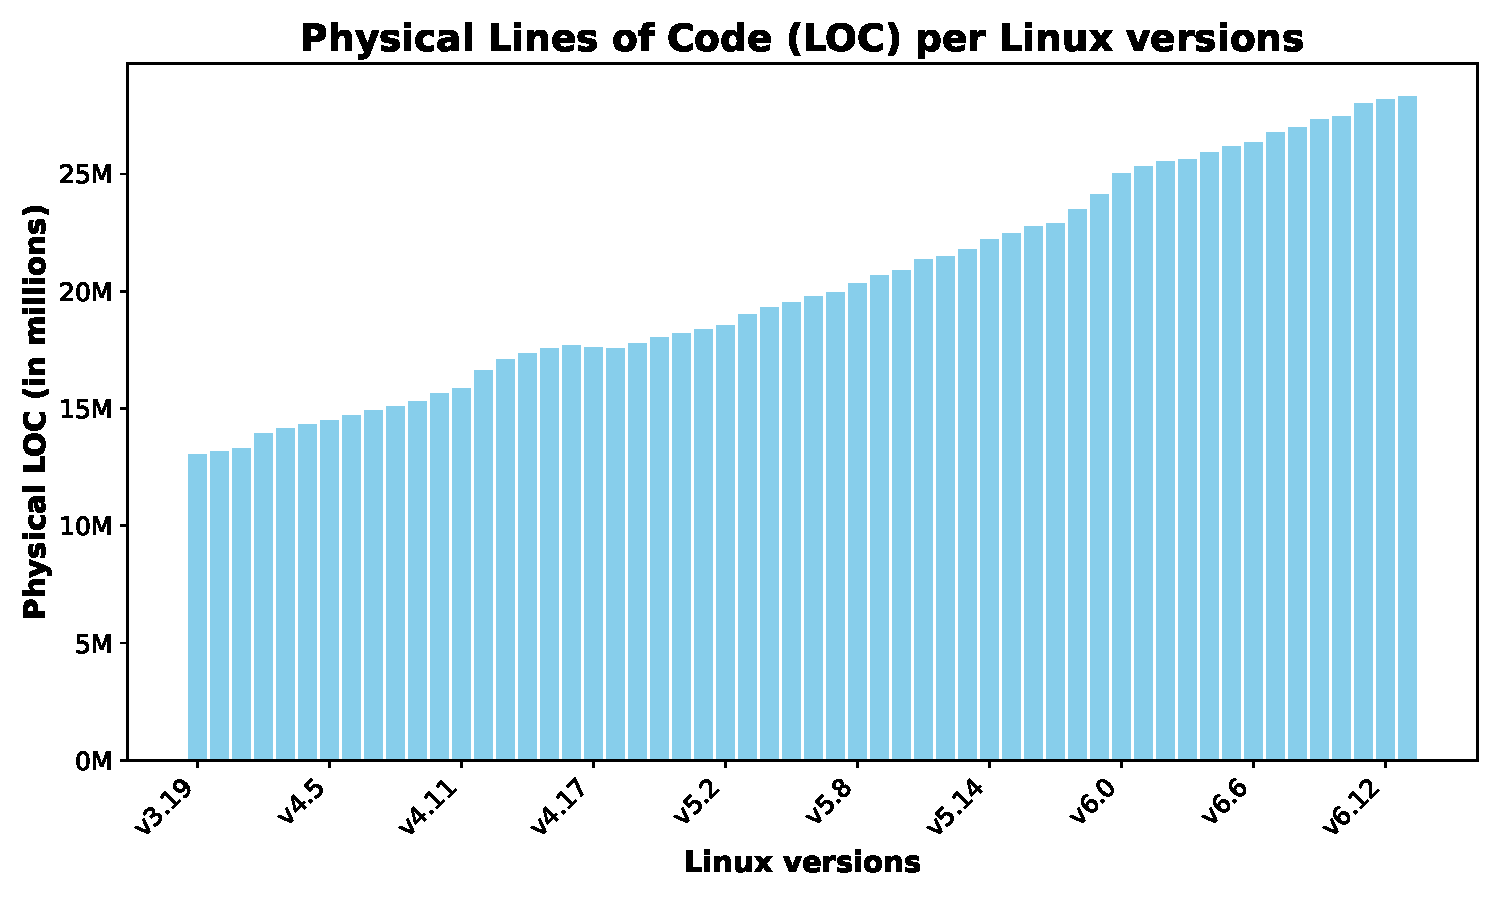
\includegraphics[width=0.75\textwidth]{images/phys-loc.pdf}
    \caption{Linux physical LOC from version 3.19 to 6.13.\label{fig:loc-linux}}
\end{figure}

\begin{figure}[h!]
    \centering
    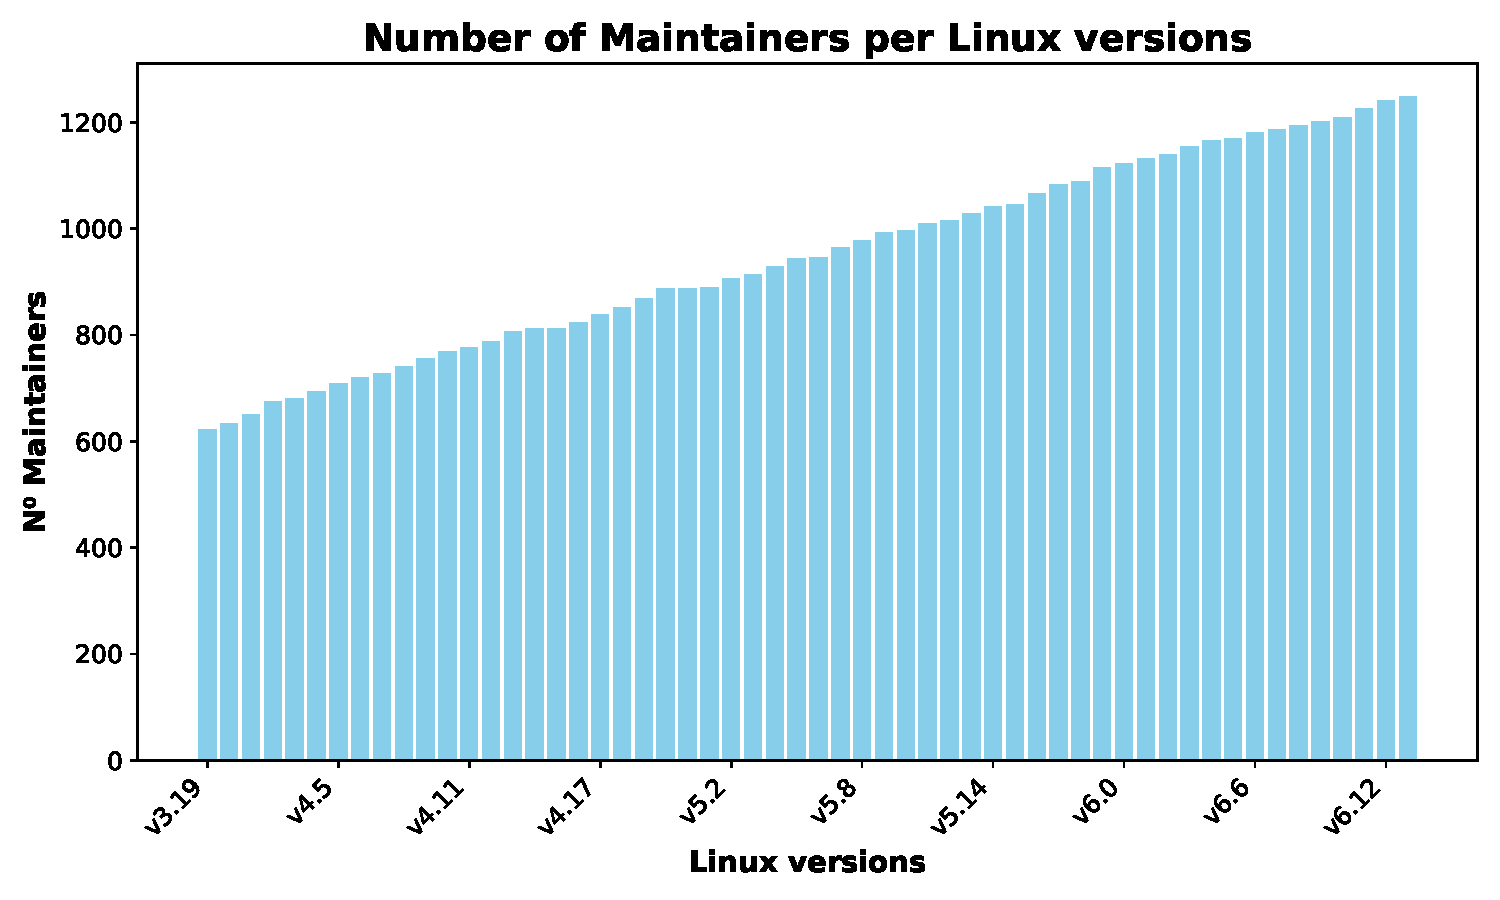
\includegraphics[width=0.75\textwidth]{images/maintainers.pdf}
    \caption{Number of Linux maintainers from version 3.19 to 6.13.\label{fig:maintainers-linux}}
\end{figure}

\begin{figure}[h!]
    \centering
    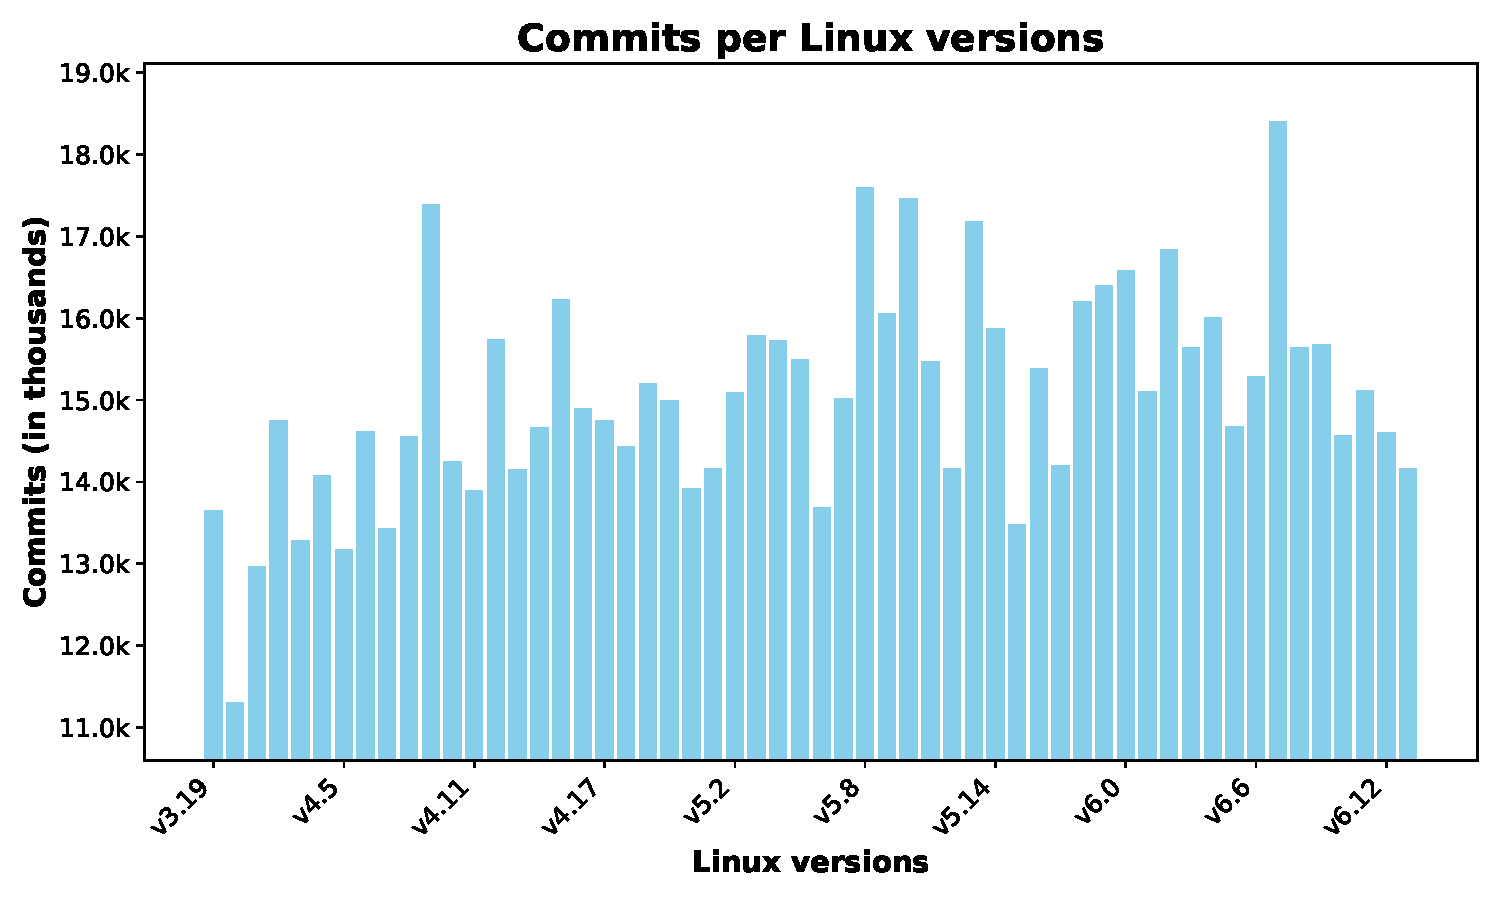
\includegraphics[width=0.75\textwidth]{images/commits.pdf}
    \caption{Commits in the development cycle of versions 3.19 to 6.13.\label{fig:commits-linux}}
\end{figure}


Figure \ref{fig:loc-linux} displays the increase of \textit{physical Lines of Code} (physical LOC)\footnote{A software metric that measures the number of source lines of code (excluding blank ones and comments) in a program source code.} and shows how the Linux kernel codebase is steadily growing regarding its size. We can derive that the project complexity is also growing as more features, drivers, and the like are continuously being merged. Interestingly, by investigating the entries in the \texttt{MAINTAINERS} file, we produced Figure \ref{fig:maintainers-linux} that depicts how the number of maintainers steadily increases.

Notwithstanding the increase in the number of maintainers, we can see in Figure \ref{fig:commits-linux} that the amount of commits in each development cycle of Linux fluctuates between 13000 and 17500 since version 3.19, excluding outliers. Every commit is different as an individual commit can be a massive change, while a set of ten commits can be a single line change ten times, and a difference of four and a half thousand commits is expressive, so we can not derive solid conclusions based on these statistics. However, just the fact that the number of commits has fluctuated consistently indicates that the contribution throughput does not scale in the same fashion as the number of maintainers.

The Linux kernel development model functions as a self-sustaining and highly specialized ecosystem. However, by extrapolating the empirical evidence, we can assume that the model reliance on a continuous influx of skilled contributors, a highly dedicated pool of maintainers, and ever-increasing code complexity suggests characteristics similar to an ``economic bubble'' where short-term growth may mask long-term sustainability risks.

\section{Research Methods}
\label{chp:research-methods}

For this proposed research, we envision a multi-method approach that is a combination of these two research methods: (i) Ethnographic Case-Studies (Participant and Non-Participant Observation) and (ii) Multivocal Literature Review.

\subsection{Ethnographic Case-Studies}

An ethnographic case study is a qualitative research approach that combines an in-depth, context-rich investigation of a specific case with ethnographic methods such as participant and non-participant observation, interviews, and document analysis. It seeks to understand social practices, cultural meanings, and lived experiences within a particular setting, emphasizing the relations between individual agency and broader structures~\cite{edmonds2017-research-design}.

As mentioned, the researchers have a vast background in academia and practice with the Linux ecosystem, firsthand or inherited from the experience of other researchers and people involved in the ecosystem. These two sources of insights are what we call \textit{Participant Observation} and \textit{Non-Participant Observation}, respectively, and together represent the primary research method of this project.

\subsubsection{Participant Observation}

In regards to the former, the aim of the participant observation is for the doctoral student to continue his involvement in the Linux project in subsystems like the AMD GPU but go deeper in terms of other subprojects (\textit{Rust for Linux}\footnote{\href{https://rust-for-linux.com/}{Rust for Linux project documentation.}} is one marked to be explored) and in terms of the impact of contributions and possibly escalating to the role of file/driver maintainer. The plan is to systematically catalog the experiences and interactions to build a contributing journal. Also, as noted, the doctoral student maintains two supporting projects for the Linux ecosystem, kw and patch-hub, which are rich sources of insights.

\subsubsection{Non-Participant Observation}

Concerning the latter, the non-participant observation comprises three complementary fronts:

\begin{enumerate}
    \item Mentor new contributors (newcomers) to the Linux ecosystem and collect data about their experience through cataloging mentors' perspectives and observations;
    \item Conduct experiments with new contributors (newcomers) to the Linux ecosystem and, in a separate trial of experiments, veteran kernel developers to qualitatively and quantitatively measure how the FLOSS tools produced cover workflows and mitigate bottlenecks. For the newcomers' trials, questionnaires will be used to collect data, while for the veteran trials, data will be collected through telemetry using an anonymization approach similar to the one used by \textit{Debian Popularity Contest}\footnote{\href{https://popcon.debian.org/}{Debian Popularity Contest website}.};
    \item Interact with key players from the Linux ecosystem and collect feedback through \textit{in-loco} participation in community events, which was a suggestion given by the board of the Linux Foundation to our research group to the detriment of conducting surveys.
\end{enumerate}

\subsection{Multivocal Literature Review}

A \textit{Multivocal Literature Review} (MLR) is a systematic approach to synthesizing knowledge from diverse sources, including academic publications, Grey Literature (GL), practitioner reports, and other non-traditional texts. Essentially combining \textit{Systematic Literature Review} (SLR) and \textit{Grey Literature Review} (GLR), it acknowledges and integrates multiple perspectives and understandings of a research topic while identifying convergence, divergence, and gaps in the discourse~\cite{vahid2018-mlr}. \textit{Wen (2021)} \cite{wen2021-masterthesis}, in her master's thesis, conducted an MLR to identify the gaps between state-of-the-art (academia understanding) and state-of-the-practice (practitioners understanding). As a secondary result, \textit{Wen (2021)} \cite{wen2021-masterthesis} used the lessons learned when conducting the GLR to devise ``guidelines to examine FLOSS projects through its community publications'' due to the lack of a consolidated method to do GLR in this specific context. We plan to make an MLR similar to how \textit{Wen (2021)} \cite{wen2021-masterthesis} did, but limiting the scope to development workflows and going back only 5 years since going back further would result in duplication of work.

The MLR will be meaningful for triangulating findings from the ethnographic case studies - our primary method - with state-of-the-art and state-of-the-practice to eliminate biases and strengthen the research.

\section{Work Plan and Execution Schedule}
\label{chp:workplan-schedule}

The work plan is to apply the two research methods as concurrently as possible while continuously developing the mentioned FLOSS tools. We divided the research work into four phases, each one producing a new iteration of the taxonomy describing the workflows of the Linux kernel development model.

\subsection{Phase I: Ethnographic Case Study I}

In the first phase, the doctoral student immersed himself not so profoundly into the Linux ecosystem by exploring the dynamics of contributing to some parts of the ecosystem and mentoring graduate and undergraduate students as newcomers. In a sense, we dip ourselves into the ecosystem while observing how the movement of new developers into it works.

\paragraph{P1.1: Exploration into the Linux ecosystem.}
The doctoral student re-acclimated himself with the Linux kernel ecosystem by sending simple and exploratory patches to the AMD GPU, IIO, and staging. He also recompiled the experiences of fellow researchers and members of the Linux community by reading their blog posts, some academic publications, and through direct conversations.

\paragraph{P1.2: Mentor newcomers I.}
In the first semester of 2024, the \textit{Free Software Development} course ministered at IME-USP dedicated the first three-fourths of the discipline program to mentoring around 30 graduated and undergraduate students that involved teaching them how to: set up a testing environment; configure, compile, install, and boot a custom Linux kernel from source code; develop changes; send changes as contributions and participate in the review process; and much more. Essentially, lead them through all the steps described in the concept map of Figure \ref{fig:patch-development-workflow}. To accomplish this, students did in-person workshops based on tutorials devised by past researchers from the Software Systems Research Group of IME-USP, who are veteran Linux developers. The doctoral student was the principal mentor in this process. At the end of the course, students filled out a survey to collect data about their experiences.

\paragraph{\underline{\textit{P1.3}}: kw/patch-hub dev I.}
kw has been in development since 2019, and it already encoded many solutions for workflows at the start of 2024. In this first phase, the doctoral student invested great effort and time in developing, maintaining, and bringing new contributors to the project. From February to August, the doctoral student was also a mentor in \textit{Google Summer of Code 2024} (GSoC 24) for two contributors in kw. The doctoral student transformed patch-hub - which was a proof-of-concept tool implemented in Bash script inside the kw codebase - into a dedicated project with its own codebase and written in Rust. During July, the doctoral student fully migrated the tool to the new project and surpassed its features, performance, and maintainability, which were unacceptable in the old form. Throughout the remainder of the second term of 2024, the project started to have recurring contributors forming a small community and really elevating it to a FLOSS project.

\subsection{Phase II: Ethnographic Case Study II}
The second phase continues the first phase, although the doctoral student deepens the immersion into the ecosystem by making more meaningful contributions and trying to be trusted with some maintainer responsibilities. Mentoring newcomers is virtually the same as in Phase I, but the researchers also conduct a first trial of experiments.\looseness=-1

\paragraph{P2.1: Deep immersion into the Linux ecosystem.}
The doctoral student submits contributions that have a more profound impact on Linux subprojects and also engages in reviews sent from other contributors. The idea is to experience the role of non-casual contributors and, at least, experience one of the major responsibilities of maintainers, which is reviewing proposed changes. Additionally, the doctoral student will try to undertake formal responsibilities as a maintainer by organically and politely escalating his importance in the subproject(s).

\paragraph{P2.2: Mentor newcomers II.}
With another offering of the Free Software Development course in the first semester of 2025, mentoring newcomers will take the same shape, apart from natural adaptations and changes that resulted from the lessons learned in the first mentoring.

\paragraph{P2.3: Conduct Experiments I (newcomers).}
In the middle of the workshop series of \textbf{P2.2}, half of the course students will be randomly selected to use kw tools from that point onwards, while the other half will maintain use of the same tools used in the first mentoring. The overall program will remain the same, diverging from the tools used. Data describing the impact of including the use of kw tools will be collected through a survey, which will enable us to derive qualitative metrics, like how well bottleneck \textit{X} of workflow \textit{Y} was mitigated by kw \textit{Z} tool(s), and also quantitative metrics like measure how much time workflow \textit{W} demanded with and without the use of kw.

\paragraph{\underline{\textit{P2.4}}: kw/patch-hub dev II.}
With a better understanding of core workflows, in the second phase, the development of kw will focus on maintaining and refining the existing features it has while making a patch-hub with features enough to be included in a developer routine. The doctoral student is, once again, mentoring a contributor in GSoC 25. However, the work is focused on patch-hub. 

\subsection{Phase III: Unbiased Perspectives}

Through ethnographic case studies, we can get valuable information from closely observing and immersing ourselves in the Linux development model. However, there are some innate biases regarding how the researchers (and their associates) view the ecosystem and the subset of the ecosystem considered. To mitigate this, triangulating these results with academic and grey literature, along with the perspective of the community and its key players, is necessary.

\paragraph{P3.1: Conduct Multivocal Literature Review.}
Here, the researchers will cross the state-of-the-art from the last 5 years about Linux kernel development, focusing on workflows, with state-of-the-practice from community publications like blog posts, articles, and mailing lists.

\paragraph{P3.2: Collect feedback from the Linux community and its key players at events.}
In previous research works done by past researchers from our research group, the board of the Linux Foundation requested that feedback from the community and key players be collected by participating in in-loco events and direct exchange instead of requesting surveys. Given this guidance, the researchers, especially the doctoral student, aim to participate in events such as \textit{FOSDEM}\footnote{\href{https://fosdem.org/2025/}{FOSDEM 2025 site.}}, as a speaker presenting the kw project and patch-hub, to interact with these sources of valuable information (which the student did on this DebConf 2025\footnote{\href{https://debconf25.debconf.org/schedule/}{DebConf 2025 schedule.}})

\paragraph{\underline{\textit{P3.3}}: kw/patch-hub dev III.} Leveraging \textbf{Taxonomy I}, incorporate its knowledge in developing kw and patch-hub.

\subsection{Phase IV: Final Validation.}
From the coalition of the results from Phase I and II with Phase III, we aim to validate our reviewed theoretical framework describing the Linux kernel development model in a real-world scenario through experiments with veteran Linux developers.

\paragraph{P4.1: Conduct Experiments II (real practitioners).}
To capture the actual workflows of practitioners, this trial of experiments will be conducted by having veteran developers follow their day-to-day tasks naturally while using kw tools and patch-hub. Data will be generated seamlessly using kw, which already keeps statistics of some actions locally, like how many times the user compiled the kernel and the minimum, maximum, and average time it took for each day or period. Data telemetry is being investigated and planned to be implemented in the project soon. It will be inspired in the \textit{Debian Popularity Contest}, where Debian users that comply send data about Debian packages to servers and go through a data anonymization process before analysis.

\paragraph{\underline{\textit{P4.2}}: kw/patch-hub dev IV.} Leveraging \textbf{Taxonomy II}, incorporate its knowledge in developing kw and patch-hub.

\subsection{Work Plan Overview}

\begin{figure}[ht]
    \centering
    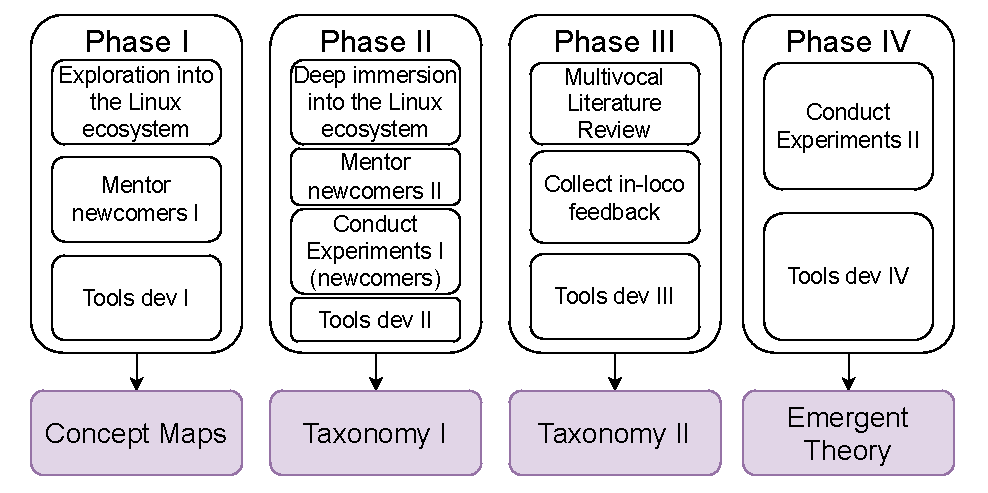
\includegraphics[width=0.8\textwidth]{images/phd-phases.pdf}
    \caption{Research work plan.\label{fig:research-work-plan}}
\end{figure}

Figure \ref{fig:research-work-plan} is a diagram that summarizes the four phases. In this figure, each phase also describes the core work it represents (blue boxes at the middle of the figure), along with the iteration of the theoretical framework produced by the phase (magenta boxes at the bottom).

\subsection{Execution Schedule}

Given the tasks of each phase, Table \ref{tab:work-plan} describes the five-year (60 months) schedule for this proposed doctoral research. \textbf{P0} refers to Phase 0 regarding the courses the doctoral student has to attend as part of his post-graduation program. For better visualization, activities in italics and underlined pertain to development tasks. Also, the cyan color represents the terms when the doctoral student plans to do a \textit{Research Internship Abroad} (RIA) to Spain at the \textit{Rey Juan Carlos University} (URJC), which is already agreed with the RIA advisor.

\begin{table}[htb]
\small
\centering
\caption{60 months schedule for the proposed doctoral research.}
\label{tab:work-plan}
\begin{tabular}{|c|c|c|c|c|c|c|c|c|c|c|}
\hline
\rowcolor{lightgray}
Activity &
\multicolumn{1}{c|}{\begin{tabular}[c]{@{}c@{}}24.1\end{tabular}} &
\multicolumn{1}{c|}{\begin{tabular}[c]{@{}c@{}}24.2\end{tabular}} &
\multicolumn{1}{c|}{\begin{tabular}[c]{@{}c@{}}25.1\end{tabular}} &
\multicolumn{1}{c|}{\begin{tabular}[c]{@{}c@{}}25.2\end{tabular}} &
\multicolumn{1}{c|}{\begin{tabular}[c]{@{}c@{}}26.1\end{tabular}} &
\multicolumn{1}{c|}{\begin{tabular}[c]{@{}c@{}}\cellcolor[HTML]{CCCCFF}26.2\end{tabular}} &
\multicolumn{1}{c|}{\begin{tabular}[c]{@{}c@{}}\cellcolor[HTML]{CCCCFF}27.1\end{tabular}} &
\multicolumn{1}{c|}{\begin{tabular}[c]{@{}c@{}}27.2\end{tabular}} &
\multicolumn{1}{c|}{\begin{tabular}[c]{@{}c@{}}28.1\end{tabular}} &
\multicolumn{1}{c|}{\begin{tabular}[c]{@{}c@{}}28.2\end{tabular}} \\ \hline
\cellcolor[gray]{0.8}\textbf{P0.0} & X & X & X & X & & \cellcolor[HTML]{CCCCFF}  & \cellcolor[HTML]{CCCCFF} &   &   & \\ \hline
\cellcolor[gray]{0.8}\textbf{P1.1} & X & X & X &   & & \cellcolor[HTML]{CCCCFF}  & \cellcolor[HTML]{CCCCFF} &   &   &   \\ \hline
\cellcolor[gray]{0.8}\textbf{P1.2} & X &   &   &   & & \cellcolor[HTML]{CCCCFF}  & \cellcolor[HTML]{CCCCFF} &   &   &   \\ \hline
\cellcolor[gray]{0.8}\underline{\textit{\textbf{P1.3}}} & X & X & & & & \cellcolor[HTML]{CCCCFF}  & \cellcolor[HTML]{CCCCFF} &   &   &   \\ \hline
\cellcolor[gray]{0.8}\textbf{P2.1} &   &   & X & X & X & \cellcolor[HTML]{CCCCFF}  & \cellcolor[HTML]{CCCCFF}  &   &   &   \\ \hline
\cellcolor[gray]{0.8}\textbf{P2.2} &   &   & X &   &   & \cellcolor[HTML]{CCCCFF}  & \cellcolor[HTML]{CCCCFF}  &   &   &   \\ \hline
\cellcolor[gray]{0.8}\textbf{P2.3} &   &   & X &   &   & \cellcolor[HTML]{CCCCFF}  & \cellcolor[HTML]{CCCCFF}  &   &   &   \\ \hline
\cellcolor[gray]{0.8}\underline{\textit{\textbf{P2.4}}} &   &   & X & X & X & \cellcolor[HTML]{CCCCFF}  & \cellcolor[HTML]{CCCCFF} &   &   &   \\ \hline
\cellcolor[gray]{0.8}\textbf{P3.1} &   &   &   &   & X & \cellcolor[HTML]{CCCCFF}X & \cellcolor[HTML]{CCCCFF}X & X &   &   \\ \hline
\cellcolor[gray]{0.8}\textbf{P3.2} &   &   & X & X & X & \cellcolor[HTML]{CCCCFF}X & \cellcolor[HTML]{CCCCFF}X &   &   &   \\ \hline
\cellcolor[gray]{0.8}\underline{\textit{\textbf{P3.3}}} &   &   &   &   & & \cellcolor[HTML]{CCCCFF}X & \cellcolor[HTML]{CCCCFF}X & X &   &   \\ \hline
\cellcolor[gray]{0.8}\textbf{P4.1} &   &   &   &   &  & \cellcolor[HTML]{CCCCFF}  & \cellcolor[HTML]{CCCCFF} & X & X &   \\ \hline
\cellcolor[gray]{0.8}\underline{\textit{\textbf{P4.2}}} &   &   &   &   &  & \cellcolor[HTML]{CCCCFF}  & \cellcolor[HTML]{CCCCFF} & X & X & X \\ \hline
\end{tabular}
\normalsize
\end{table}

\section{Publications}
\label{sec:publications}

In this section, we present the student's publications. Below is a list of eight accepted papers where the student had some authorship role\footnote{All accepted publications are directly related to or stem from the research work presented in this proposal, even those where the student is on the record as a co-author.}:

{\footnotesize
\begin{itemize}
    \item \textbf{D. Tadokoro}, R. Siqueira, and P. Meirelles, \textit{Kworkflow: a Linux kernel Developer Automation Workflow System}. In \textit{39th Brazilian Symposium on Software Engineering - Tools Track}.
    \item \textbf{D. Tadokoro} and P. Meirelles, \textit{Can the Linux kernel sustain 30 more years of growth? Toward mitigating bottlenecks in its development model}. In \textit{39th Brazilian Symposium on Software Engineering - Insightful Ideas and Emerging Results Track}.
    \item \textbf{D. Tadokoro}, R. Passos, and P. Meirelles, \textit{Guidelines for Boosting Long-Lasting FLOSS Contributors}. In \textit{DebConf 2025 - Academic Track}.
    \item \textbf{D. Tadokoro}, E. Mendes, and P. Meirelles, \textit{Estudo, implementação e análise de estratégias para simplificar o modelo de contribuição do kernel Linux}. In \textit{32º Simpósio Internacional de Iniciação Científica e Tecnológica da USP Universidade de São Paulo}.
    \item R. Passos, A. Pilone, \textbf{D. Tadokoro}, and P. Meirelles, \textit{Streamlining Analysis on the Linux project with DUKS}. In \textit{VISSOFT 2025 - Visualization Challenge}.
    \item L. Arcanjo, \textbf{D. Tadokoro}, and P. Meirelles, \textit{ArKanjo: a tool for detecting function-level Code Duplication in the Linux Kernel}. In \textit{DebConf 2025 - Academic Track}.
    \item \textbf{D. Tadokoro} and P. Meirelles, \textit{Estratégias de ensino para incentivar a participação consistente em projetos de Software Livre}. In \textit{13th Workshop on Software Visualization, Evolution and Maintenance}.
    \item R. Passos, A. Pilone, \textbf{D. Tadokoro}, and P. Meirelles, \textit{DUKS: visualizações e análises unificadas para o Kernel Linux}. In \textit{13th Workshop on Software Visualization, Evolution and Maintenance}.
\end{itemize}
}
Beyond accepted publications, there are two works in progress to be submitted to the \textit{International Conference on Software Engineering 2026 - Software Engineering Education and Training (ICSE 2026 - SEET)} and the journal \textit{Information and Software Technology (IST)}.


\printbibliography
\end{document}
